\subsection{Chaos-Test}
Bei den Chaos-Tests werden die Ergebnisse der Szenarien auf der Haupt-API vorgestellt.
Dabei werden die wichtigsten Testdaten zur Bestimmung der Zuverlässigkeit jedes Testdurchlaufs präsentiert.
Die angezeigten Werte sind eine Aggregation aller Testdurchläufe.
Einerseits wird gezeigt, wie durchschnittlich verfügbar die Anwendung während des Tests war.
Die durchschnittliche Fehlerrate wird ebenfalls bewertet.
Dazu kommt, wie lange das System im Durchschnitt gebraucht hat, um die Services wiederherzustellen, und bei wie vielen Testdurchläufe die Umgebungen innerhalb eines Test dies hinbekommen haben.

Zum Schluss jedes Szenarios wird die Auswertung jedes Testdurchlaufs angezeigt und wie der durchschnittliche Score der Testdurchläufe war.

\subsubsection{Teilausfall bei der Haupt-API}

Bei einem Teilausfall der Haupt-API hat die Docker-Compose-Umgebung es bei keinem Testdurchlauf geschafft, den Service innerhalb des Testfensters selbst wiederherzustellen, wie in der Tabelle \ref{tab:chaos_api_instance_down} zu sehen ist.
Dadurch hat Docker keinen der Tests bestanden, weshalb der Zuverlässigkeits-Score der Docker-Compose-Umgebung bei jeder Testumgebung eine 0 beträgt, wie in Abbildung \ref{fig:chaos_api_instance_down} zu sehen ist. 
Die k3s-Umgebung hat dagegen jeweils einen Score von 60 Punkten oder mehr erzielt.
Zur Wiederherstellung des Services hat k3s im Durchschnitt weniger als eine Sekunde gebraucht. Da die Docker-Compose-Umgebung den Service nicht von selbst wiederherstellen konnte, wurde keine Zeit eingetragen, da diese nur die Länge vom Chaos-Anfang bis Testende betragen würde. 
\begin{table}[htbp]
\centering
\caption{Vergleich der Chaos-Test-Metriken bei Teilausfall der Haupt-API}
\label{tab:chaos_api_instance_down}

\begin{tabular}{lrr}
\toprule
\textbf{Metrik} & \textbf{Docker} & \textbf{K3s} \\
\midrule
Error Rate [\%]         & 98.96 & 3.11 \\
Availability [\%]       & 1.04 & 96.89 \\
Recovery Time [s]      & - & 0.44 \\
Recovered [Anzahl]      & 0 & 3 \\
\bottomrule
\end{tabular}

\end{table}

\begin{figure}[htbp]
\centering
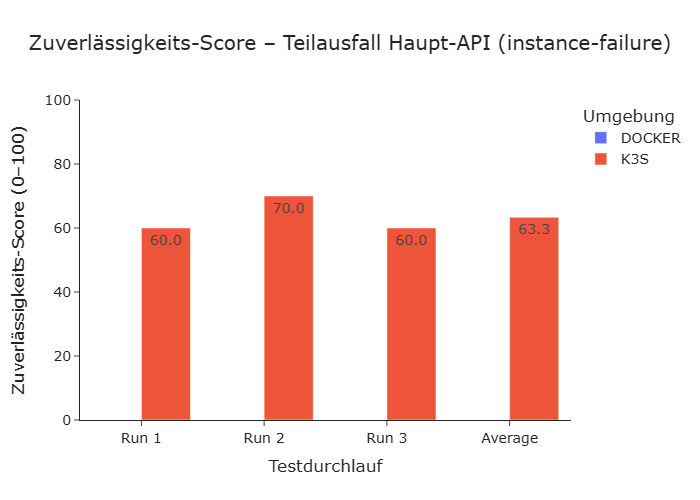
\includegraphics[width=0.8\textwidth]{bilder/tests/reliability_score_api-instance-down_instance-failure.png}
\caption{Zuverlässigkeit Score bei Teilausfall der Haupt-API}
\label{fig:chaos_api_instance_down}
\end{figure}
\FloatBarrier
\subsubsection{Komplettausfall der Haupt-API}
Bei einem Komplettausfall der Haupt-API hat die Docker-Compose-Umgebung es wieder nicht hinbekommen, den Service von selbst wiederherzustellen. Deshalb hat die Docker-Compose-Umgebung in der Abbildung \ref{fig:chaos_api_outage} in jedem Testdurchlauf 0 von 100 Punkten.
Der Score von Kubernetes beträgt bei jedem Testdurchlauf 35 von 100.
In der Tabelle \ref{tab:chaos_api_outage} ist zu sehen, dass die k3s-Umgebung eine niedrige Verfügbarkeit und eine höhere Fehlerrate hatte.
Die k3s-Umgebung hat im Durchschnitt unter zwanzig Sekunden benötigt, um den Service wiederherzustellen. 
Da die Docker-Compose-Umgebung es nicht innerhalb des Testfensters geschafft hat, den Service wiederherzustellen, wurde keine Zeit eingetragen, da diese nur die Zeit vom Chaos-Anfang bis Testende darstellen würde.

\begin{table}[htbp]
\centering
\caption{Vergleich der Chaos-Test-Metriken bei Komplettausfall der Haupt-API}
\label{tab:chaos_api_outage}

\begin{tabular}{lrr}
\toprule
\textbf{Metrik} & \textbf{Docker} & \textbf{K3s} \\
\midrule
Error Rate [\%]                    & 98.97 & 5.63 \\
Availability [\%]                & 1.03 & 94.37 \\
Recovery Time [s]                 & - & 17.29 \\
Recovered [Anzahl]                 & 0 & 3 \\
\bottomrule
\end{tabular}

\end{table}

\begin{figure}[htbp]
\centering
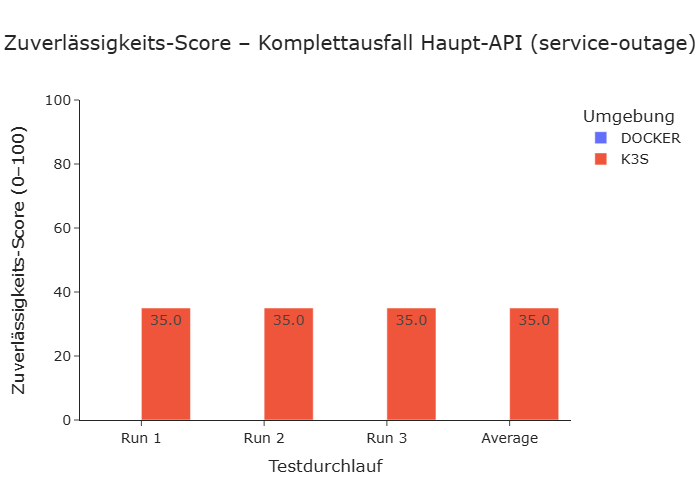
\includegraphics[width=0.8\textwidth]{bilder/tests/reliability_score_api-outage_service-outage.png}
\caption{Zuverlässigkeit Score bei Komplettausfall der Haupt-API}
\label{fig:chaos_api_outage}
\end{figure}
\FloatBarrier
\subsubsection{Update der Haupt-API}
Bei einem Update der Haupt-API hat die Docker-Compose-Umgebung in jedem Testlauf den Score 35 von 100 erzielt, während die k3s-Umgebung mit dem Score 70 von 100 in jedem Testlauf das Doppelte erreicht hat.
In der Tabelle \ref{tab:chaos_api_update} benötigte die Docker-Compose-Umgebung im Durchschnitt 21,38 Sekunden, um den Service wiederherzustellen, während es bei der k3s-Umgebung zu keinem Ausfall kam.
\begin{table}[htbp]
\centering
\caption{Vergleich der Chaos-Test-Metriken bei Update der Haupt-API}
\label{tab:chaos_api_update}

\begin{tabular}{lrr}
\toprule
\textbf{Metrik} & \textbf{Docker} & \textbf{K3s} \\
\midrule
Error Rate [\%]                    & 7.76 & 3.12 \\
Availability [\%]                & 92.24 & 96.88 \\
Recovery Time [s]       & 21.38 & 0.00 \\
Recovered [Anzahl]  & 3 & 3 \\
\bottomrule
\end{tabular}

\end{table}

\begin{figure}[htbp]
\centering
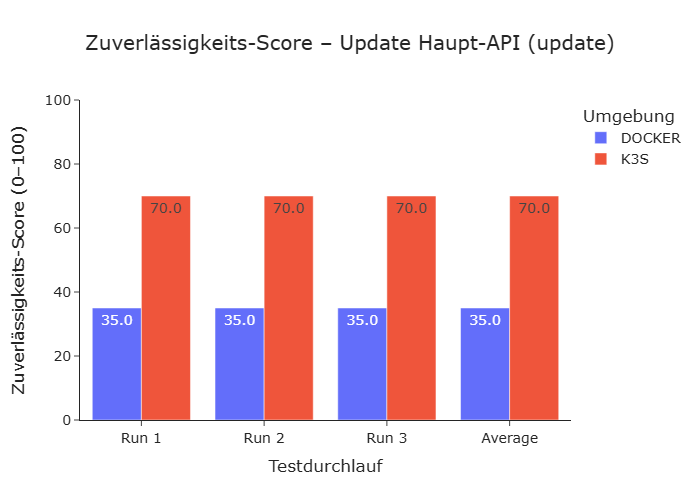
\includegraphics[width=0.8\textwidth]{bilder/tests/reliability_score_api-update_update.png}
\caption{Zuverlässigkeit Score bei Update der Haupt-API}
\label{fig:chaos_api_update}
\end{figure}
\FloatBarrier